\documentclass{article}
\usepackage{graphicx}
\usepackage{hyperref}
\usepackage{amsmath}
\usepackage{enumitem}
\usepackage{booktabs}
\usepackage{multirow}
\usepackage{subcaption}


\title{LLM Anonymization Techniques Recommender for Datasets (LLMANO-2)}
\author{Amin Akziz, Leander Ziehm, Azbabanu Engineer, Santiago Lema}
\date{July 2025}

\usepackage[a4paper, margin=1in]{geometry}

\usepackage{setspace}
\onehalfspacing

\begin{document}

\maketitle

\begin{center}
\begin{minipage}{0.85\textwidth}
\section*{Abstract}
The need for anonymizing datasets has grown significantly with the proliferation of machine learning and large language models (LLMs). However, many users lack a clear understanding of how to properly anonymize their data without significantly compromising its utility. In response to this challenge, we present LLMANO-2, a recommender system that leverages LLMs to guide users in anonymizing CSV datasets while preserving predictive performance. Our system provides tailored recommendations based on the specific characteristics of each dataset, aiming to strike a balance between privacy and usability. The motivation for this work stems from recent data privacy incidents that highlight the risks of improper anonymization and the growing demand for practical, intelligent tools to support privacy-aware data publishing.
\end{minipage}
\end{center}

\section{Introduction}

In today’s era of big data and artificial intelligence, vast amounts of personal and sensitive information are being collected and analyzed. This increase in data collection has made dataset anonymization a critical concern, as organizations must protect individual privacy while still deriving value from the data.

Notably, data anonymization is not just a best practice but often a legal requirement; privacy regulations like the EU’s General Data Protection Regulation (GDPR) and the California Consumer Privacy Act (CCPA) mandate that personal data be anonymized or otherwise protected if it’s to be used beyond its original purpose. Failure to properly anonymize data can lead to severe regulatory penalties as well as loss of user trust.

Recently, advances in Artificial Intelligence have introduced new possibilities for smarter anonymization approaches. In particular, Large Language Models (LLMs) offer a promising approach to tackle the privacy-utility trade-off. In alignment with these developments, our work proposes LLMANO-2, an LLM-powered anonymization technique-based recommender for datasets. LLMANO-2 is designed to assist users in anonymizing tabular datasets by recommending appropriate techniques for each column of data. For a given dataset, the system leverages an LLM to analyze the column contents and identify which fields are likely sensitive and suggest how to transform or mask them. The recommendations aim to maximize privacy protection while minimizing the impact on the dataset’s utility for analysis or machine learning tasks. In the following sections we describe the architecture and methodology behind LLMANO-2, including how it processes datasets, generates anonymization recommendations, and evaluates the effectiveness of those recommendations.


\section{Background and Theory}

A dataset (for example, a CSV file or database table) typically consists of many records (rows) with multiple attributes (columns) describing each record. These attributes can include direct identifiers (such as names, email addresses, or national ID numbers) as well as indirect identifiers (such as dates of birth, gender, or ZIP codes) that might not identify someone on their own, but could do so when combined with other information.

Data anonymization refers to the process of modifying a dataset to remove or obscure personal identifiers so that individuals cannot be readily identified. It involves erasing or encrypting identifiers that connect an individual to stored data while retaining the data’s overall usefulness. The challenge is to ensure privacy without significantly degrading the utility of the data.

In practice, anonymization techniques may include removing or masking direct personal identifiers, generalizing values (for example, replacing an exact age with an age range), or pseudonymizing data by replacing real identifiers with artificial codes. These transformations allow organizations to use data for insights without exposing specific individuals.

\begin{figure}[h]
    \centering
    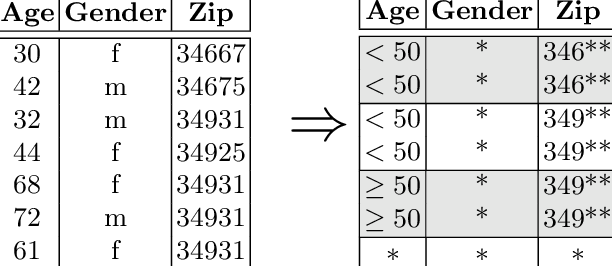
\includegraphics[width=0.65\linewidth]{images/figure1.png}
    \caption{Example of an anonymization technique applied to a simple dataset}
    \label{fig:anonymization-example}
\end{figure}

This is especially important when sharing datasets with third parties or releasing them publicly for research, as it enables data sharing and collaboration without compromising confidentiality.

Despite its importance, effective anonymization can be challenging. Research has shown that improperly anonymized datasets can still compromise privacy. Certain attributes are extremely sensitive, and even "anonymized" data can be re-identified. A famous statistic by Latanya Sweeney demonstrated that 87\% of the U.S. population could be uniquely identified using only three pieces of information, birth date, gender, and ZIP code, highlighting how a few quasi-identifiers can pinpoint individuals.

Another example where personal data was compromised is in the Netflix Prize dataset released in 2006, which contained movie ratings with personal identities removed, researchers were able to re-identify specific users by correlating the anonymized ratings with public information on IMDb (Internet Movie Database). This meant that personal viewing preferences (and even sensitive attributes inferred from them) of certain Netflix users became public, despite Netflix’s attempt to anonymize the data.

These cases show that simply removing obvious identifiers is often not sufficient. If enough data remains, determined adversaries can link supposedly anonymous records back to real individuals. Beyond the harm to individuals (such as exposing health information, financial status, or location history), such incidents expose organizations to legal liabilities and reputational damage. As data mining and cross-referencing techniques grow more sophisticated, re-identification attacks are becoming easier and more common. This puts pressure on data publishers to adopt stronger anonymization measures than were needed in the past.

At the same time, anonymization must be done carefully to preserve the usefulness of data. Over-aggressive anonymization, such as deleting or randomizing too many fields, can render a dataset nearly useless for analysis or model training, defeating the purpose of sharing the data. The more we strip away or distort to protect privacy, the less accurate or insightful the dataset becomes. A core challenge is finding the sweet spot where sensitive details are well-protected, yet the dataset still supports meaningful insights or predictions.

Achieving this balance often requires expertise and context, deciding which attributes to generalize or mask, and to what extent, without degrading the data’s integrity. Unfortunately, many users and organizations lack a clear understanding of how to achieve this. Choosing the right anonymization techniques depends on the data content, possible auxiliary data an attacker may use, and the intended use of the anonymized dataset. As a result, there is a growing need for tools and guidance to help data owners navigate this complexity.



\subsection{Identifiers and Quasi-Identifiers}

A central component in assessing the effectiveness of anonymization is understanding the adversary model, that is, what an attacker might already know and how they might use that information. Most privacy frameworks assume that adversaries possess auxiliary information such as partial datasets, public records, or domain knowledge, which they can use to link quasi-identifiers in an anonymized dataset back to specific individuals. This modeling of re-identification risk is crucial because it highlights the limitations of naive anonymization, without a formal privacy model, it is impossible to quantify the likelihood of a privacy breach. Techniques such as $k$-anonymity, $l$-diversity, and $t$-closeness each rely on different assumptions about adversary knowledge and goals. By integrating these models into anonymization strategies, systems can offer stronger, quantifiable privacy guarantees. Our work adopts this perspective by incorporating formal risk metrics directly into the anonymization recommendation process.


To give a broader context, we first define key terms related to data anonymization.
\textbf{Identifiers} are attributes in a dataset that can be used to uniquely identify an individual. They can be classified into two main categories:

\begin{itemize}
\item \textbf{Direct Identifiers} are attributes that can uniquely identify an individual without external information. Common examples include names, social security numbers, or email addresses.

\item \textbf{Indirect Identifiers}, also called \textit{quasi-identifiers}, are attributes that do not uniquely identify an individual on their own but can do so when combined with other quasi-identifiers. Examples include age, ZIP code, and gender.
\end{itemize}




\subsection{Anonymization Techniques}

Several anonymization techniques have been developed to reduce the risk of re-identification while maintaining the utility of data. These techniques vary in complexity and suitability depending on the nature of the dataset and the privacy requirements.

\begin{itemize}
\item \textbf{Suppression} involves removing data entirely from a dataset. For example, if a particular ZIP code is too rare and could identify someone, it might be deleted or replaced with a placeholder (e.g., “***”). This method is straightforward but can result in significant data loss if overused.

\item \textbf{Generalization} replaces specific values with broader categories. For instance, replacing an exact age of 29 with an age range such as “20–30,” or converting a full date of birth into just a year. Generalization helps reduce uniqueness in the data and is often used in combination with other techniques.

\item \textbf{Differential Privacy} takes a different approach by introducing mathematical noise to the data or the results of queries on the data. It provides strong theoretical guarantees that the inclusion or exclusion of a single individual’s data does not significantly affect the output, making it extremely difficult to infer information about any individual. Differential privacy is especially useful in scenarios involving aggregate data analysis or interactive queries.

\end{itemize}

These techniques are often used in combination and must be tailored to the specific context of the dataset. The choice of technique involves trade-offs between privacy protection and data utility, and selecting the appropriate method requires a clear understanding of the risks, the data's structure, and its intended use.


We also discuss user-driven anonymization processes and the limitations of manual or rule-based methods in ensuring privacy. In the remainder of this section, we outline the mathematical foundations underlying key privacy, preserving techniques in data publishing, including $k$-anonymity, $l$-diversity, and generalization strategies.

\subsection{$k$-Anonymity}

The concept of $k$-anonymity, introduced by Sweeney, is one of the foundational principles for privacy protection. A dataset is said to satisfy \textbf{$k$-anonymity} if each record is indistinguishable from at least $k-1$ other records with respect to the quasi-identifiers.

Formally, given a dataset $D$ with quasi-identifier attributes $Q_1, Q_2, ..., Q_m$, let $\pi$ be a projection onto the quasi-identifier space:

$$
\pi(D) = \{ (q_1, q_2, ..., q_m) \mid (q_1, ..., q_m) \in D \}
$$

Let $E$ be an equivalence class of records in $D$ that share the same quasi-identifier values:

$$
E = \{ r \in D \mid \forall i, \; r[Q_i] = v_i \}
$$

Then $D$ satisfies $k$-anonymity if:

$$
\forall E \subseteq D, \quad |E| \geq k
$$

This ensures that an adversary cannot link any given record to fewer than $k$ individuals. However, $k$-anonymity alone does not prevent \textit{attribute disclosure}—when sensitive values within a group are too homogeneous.

\subsection{$l$-Diversity }

$l$-Diversity extends $k$-anonymity to protect against attribute disclosure by ensuring that each equivalence class has at least $l$ ``well-represented'' sensitive attribute values.

\paragraph{ Definition.}
An equivalence class $E$ is said to have \textit{distinct $l$-diversity} if it contains at least $l$ distinct values for the sensitive attribute $S$:

\[
|\{ s_i \mid s_i \in E \}| \geq l
\]

where $s_i$ denotes the sensitive value of record $i$ in equivalence class $E$.

\paragraph{Variants.}
\begin{itemize}
    \item \textbf{Distinct $l$-diversity:}
    \[
    |\{ s_i \}| \geq l
    \]
    Requires at least $l$ distinct sensitive values, regardless of their distribution or meaning.

    \item \textbf{Entropy $l$-diversity:}
    Defines diversity using entropy of the sensitive value distribution within $E$:
    \[
    H(E) = - \sum_{s \in S} p_s \log p_s \geq \log l
    \]
    where $p_s$ is the fraction of records in $E$ with sensitive value $s$. This ensures a balanced distribution.

    \item \textbf{Recursive (c, $l$)-diversity:}
    Limits the dominance of the most frequent sensitive value. Formally, for the sorted frequencies $f_1, f_2, ..., f_m$:
    \[
    f_1 < c \cdot (f_l + f_{l+1} + ... + f_m)
    \]
    where $c$ is a parameter controlling strictness. This prevents a single sensitive value from overwhelming others even if there are $l$ distinct values.
\end{itemize}

\paragraph{Why Needed.}
While $k$-anonymity prevents identity disclosure, it does not prevent attribute disclosure if all records in an equivalence class share the same sensitive value. $l$-Diversity mitigates this by ensuring diversity in sensitive attributes.

\paragraph{Limitations.}
\begin{enumerate}
    \item \textbf{Skewness Attack.} If the overall distribution is skewed (e.g. 99\% flu, 1\% cancer), $l$-diversity fails to prevent inference because the presence of rare values remains revealing.

    \item \textbf{Similarity Attack.} Even if an equivalence class has $l$ distinct sensitive values, if they are semantically similar (e.g. different types of cancer), meaningful privacy is not protected.
\end{enumerate}


\subsection{$t$-Closeness }

$t$-Closeness improves upon $l$-diversity by protecting against attribute disclosure through distributional similarity constraints.
\paragraph{ Definition.}
An equivalence class $E$ is said to have \textit{$t$-closeness} if the distance between the distribution of the sensitive attribute within $E$ ($P_E$) and the global distribution ($P_T$) is no more than a threshold $t$:

\[
D(P_E, P_T) \le t
\]

where:
\begin{itemize}
    \item $P_E$ is the probability distribution of sensitive attribute values in equivalence class $E$
    \item $P_T$ is the global distribution of the sensitive attribute in the entire dataset
    \item $D(\cdot)$ is a chosen distance measure, typically Earth Mover's Distance (EMD) or Kullback-Leibler Divergence.
\end{itemize}

\paragraph{Motivation.}
$l$-Diversity fails if equivalence class distributions are skewed compared to the overall data, enabling attribute inference attacks. $t$-Closeness mitigates this by bounding the distributional distance.

\paragraph{Common Distance Measures.}
\begin{itemize}
    \item \textbf{Earth Mover's Distance (EMD):} Measures the minimum amount of ``work'' required to transform one distribution into another, considering attribute semantics. It is formally defined as:
    \[
    EMD(P_E, P_T) = \inf_{\gamma \in \Gamma(P_E, P_T)} \int |x-y| d\gamma(x,y)
    \]
    where $\Gamma(P_E, P_T)$ is the set of all joint distributions with marginals $P_E$ and $P_T$.

    \item \textbf{Kullback-Leibler (KL) Divergence:}
    \[
    D_{KL}(P_E || P_T) = \sum_{i} p_E(i) \log \frac{p_E(i)}{p_T(i)}
    \]
    Note: KL-divergence is asymmetric and unbounded, limiting its practical use in $t$-closeness.

\end{itemize}

\paragraph{Example.}
If the global distribution is:
\[
P_T = \{ \text{Disease A}: 95\%, \text{Disease B}: 5\% \}
\]
but an equivalence class $E$ has:
\[
P_E = \{ \text{Disease B}: 100\% \}
\]
then even with $l$-diversity, an attacker learns an individual's disease with certainty. $t$-Closeness prevents this by ensuring $P_E$ remains close to $P_T$ within threshold $t$.

\paragraph{Advantages.}
\begin{itemize}
    \item Addresses both identity and attribute disclosure by enforcing global distribution similarity.
    \item Reduces risk of skewness and similarity attacks inherent to $l$-diversity.
\end{itemize}

\paragraph{Limitations.}
\begin{enumerate}
    \item \textbf{Utility Loss:} Strict $t$-closeness often requires heavy generalization or suppression, degrading data utility.
    \item \textbf{Threshold Selection:} Choosing an appropriate $t$ balancing privacy and utility is challenging.
    \item \textbf{Implementation Complexity:} Calculating EMD for categorical attributes requires defining semantic distances or hierarchies between categories.
    \item \textbf{Overprotection:} May restrict data utility disproportionately compared to marginal privacy gains in some contexts.
\end{enumerate}


\section{Architecture}
\label{sec:architecture}

\subsection{Design rationale}

LLMANO runs on-premise and helps non-experts anonymise tabular data through natural-language interaction.  
The system must therefore (i) accept free-text questions, (ii) load a CSV file, (iii) perform an automatic privacy check before any user action, and (iv) offer callable tools so the language model can compute metrics such as $k$-anonymity or $l$-diversity when needed.  
These requirements favour a modular layout: new features should be added without modifying unrelated parts of the code.  
All major support libraries are open-source; the only closed component may be the language model itself.  
An Ollama adapter is provided so that users can connect to a local, fully open model if required.

The platform is model-agnostic.  
An abstract class \texttt{BaseLLM} exposes only the low-level operations needed by the rest of the application, such as text generation and tool invocation.  
Concrete subclasses, called adapters, hide provider-specific details like authentication and function-calling syntax.  
When a new model is added, only a new adapter is required.  
Higher-level utilities such as \texttt{fuzzy\_match} are implemented outside \texttt{BaseLLM} and rely solely on its primitives, so they work with every adapter.

\begin{figure}[h]
    \centering
    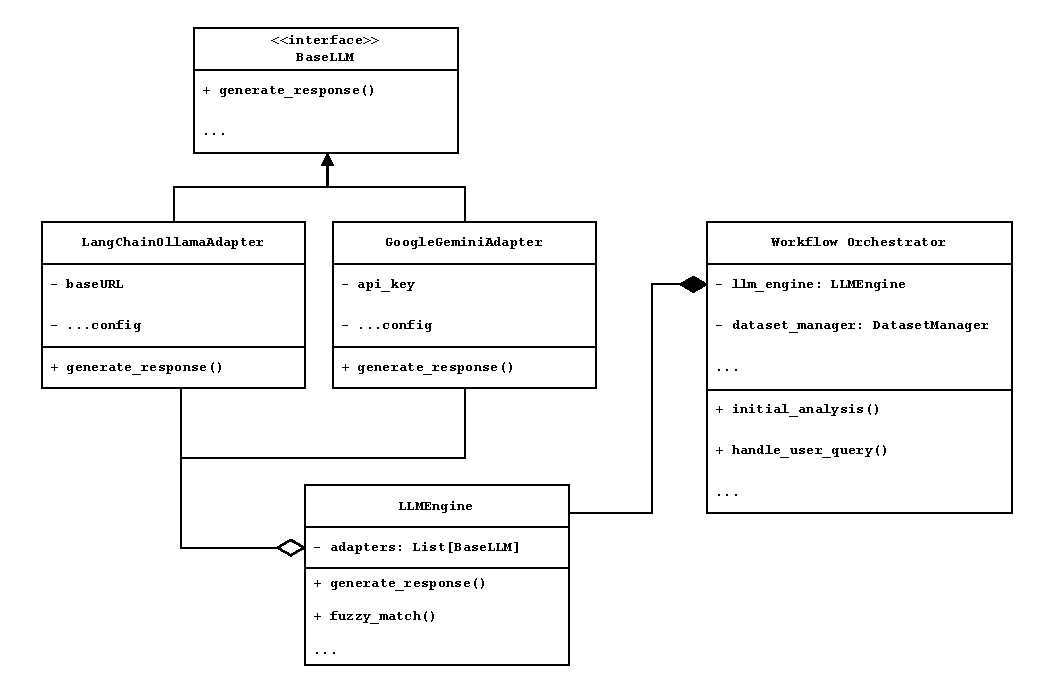
\includegraphics[width=0.8\linewidth]{images/class_diagram.pdf}
    \caption{Class diagram of \texttt{BaseLLM}, its adapters, and the orchestration layer.}
    \label{fig:class-diagram}
\end{figure}

\subsection{Hardware notes}

Resource use scales with the size of the chosen model.  
All tests have been run on Linux.  
A local 8-billion-parameter Llama model is usable on a modern desktop CPU, but responses are slow; GPU support or a smaller checkpoint is recommended.  
Measured runtimes appear in Section~\ref{evaluation}.

\subsection{LLM-mediated decisions}

Most privacy actions map an attribute to a label: direct identifier (DI), quasi-identifier (QI), sensitive attribute (SA) or non-identifier (NI).  
The helper \texttt{fuzzy\_match} performs this task by combining a natural-language context, a codebook and sample values.  
Structured output is enforced with LangChain and Pydantic, which yields reliable JSON without heavy prompt engineering.

\subsection{Workflow}

The session starts with an intake form.  
The system then profiles the file, shows a brief overview, classifies each column and suggests an anonymisation method.  
After this initial step, the user interacts through a chat window.  
If the request references a supported metric, the adapter calls the matching Python routine and includes the result in the reply.  
After every turn the model proposes three follow-up questions based on the entire conversation.

\begin{figure}[h]
    \centering
    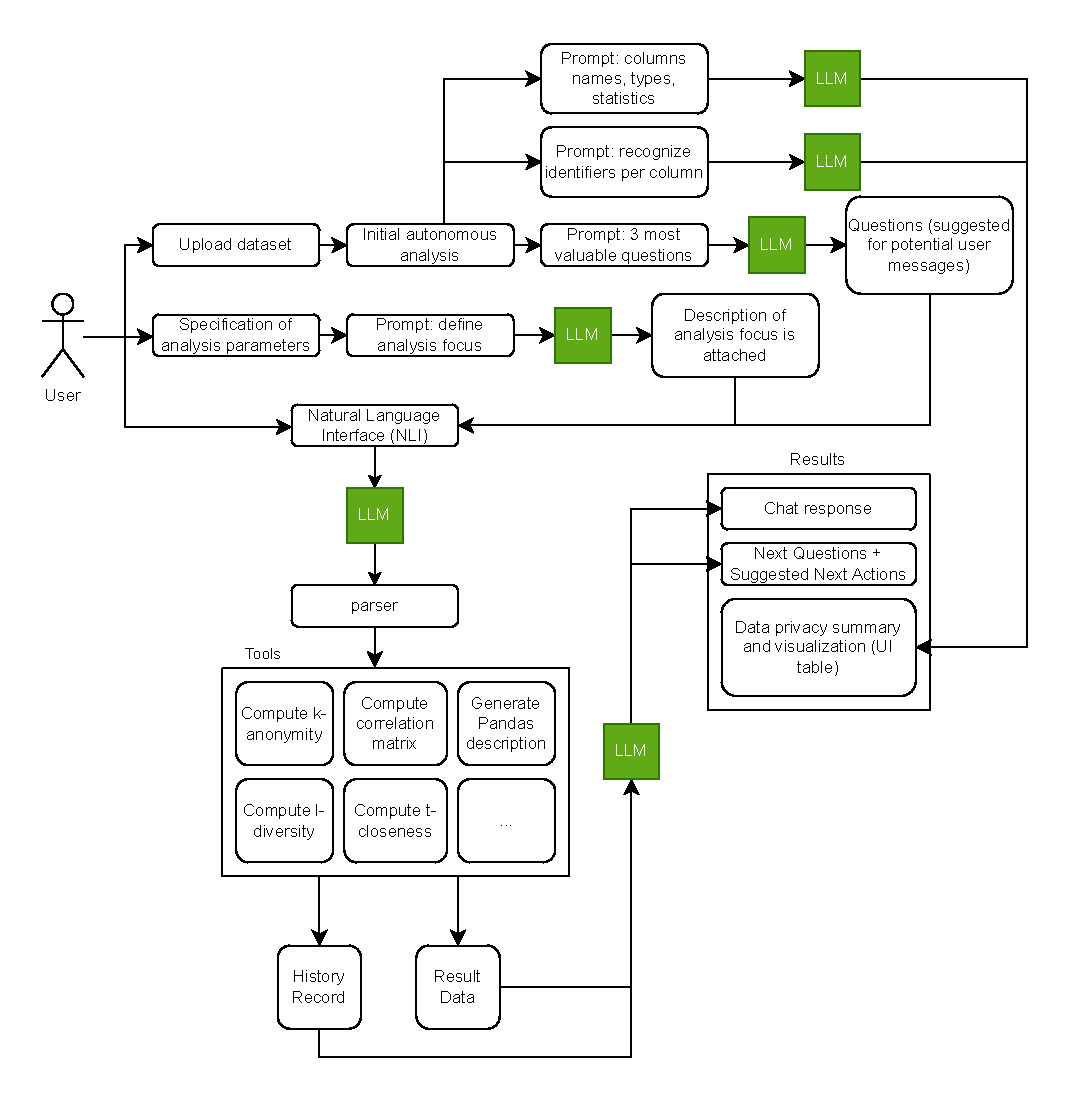
\includegraphics[width=0.85\linewidth]{images/workflow_diagram.pdf}
    \caption{Main workflow of LLMANO.}
    \label{fig:workflow-diagram}
\end{figure}

The interface displays the chat, a colour-coded table head, and a panel that lists one anonymisation method for each non-NI column.

\subsection{Summary}

The architecture meets the design goals: it runs locally, screens the data automatically and answers natural-language queries.  
Modularity is achieved through the adapter layer, and structured outputs ensure that the application receives well-formed data.  
The system can be extended without exposing raw records.

% ------------------------------------------------------------------
\section{User Interface}
\label{sec:ui}

The interface guides the user through three screens: upload, context, and analysis.  
The layout is simple so that colour is reserved for risk levels.

\subsection{Upload screen}

The first page asks the user to drag and drop a CSV file and to select a language model (Figure~\ref{fig:ui-upload}).  
No data are sent to the back-end until the file selection is confirmed.

\begin{figure}[h]
    \centering
    %
    \begin{minipage}[c]{0.48\linewidth}
        \centering
        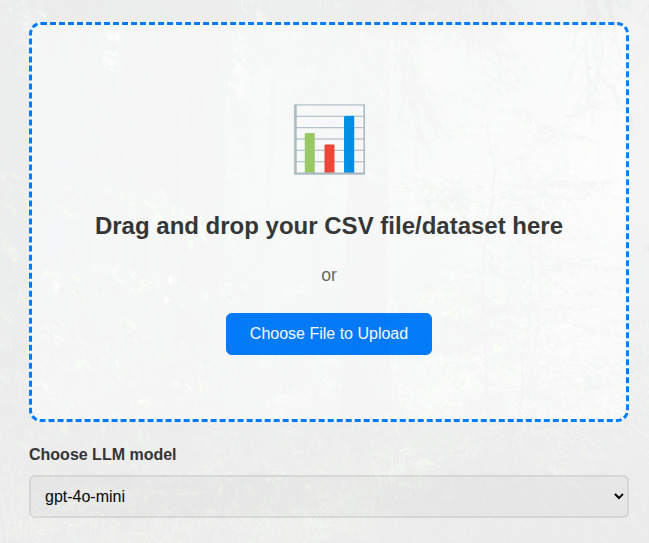
\includegraphics[height=7cm]{images/upload_ui.jpg}
        \subcaption{Upload screen with file selector and model drop-down.}
        \label{fig:ui-upload}
    \end{minipage}\hfill
    %
    \begin{minipage}[c]{0.48\linewidth}
        \centering
        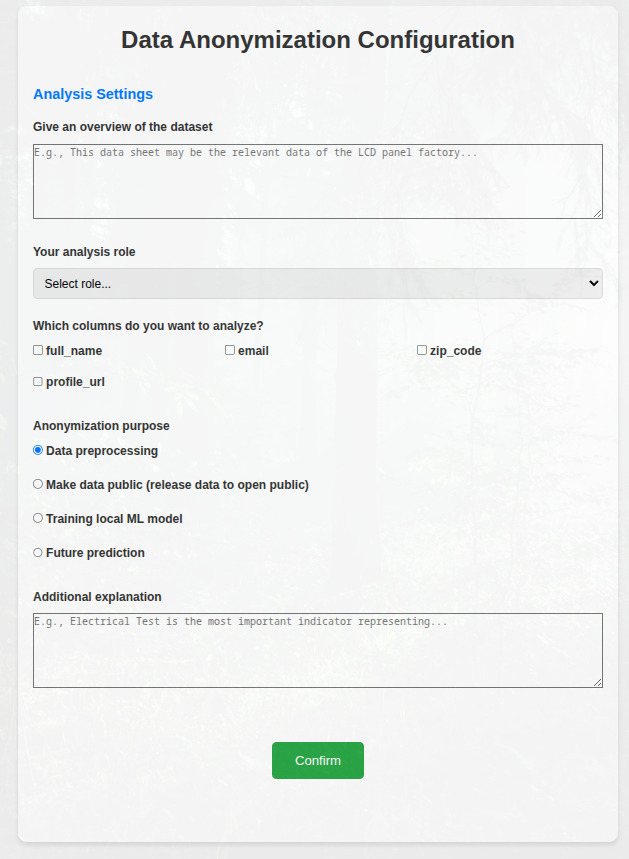
\includegraphics[height=9cm]{images/form_ui.jpg}
        \subcaption{Context form for analysis purpose and attribute selection.}
        \label{fig:ui-context}
    \end{minipage}
    %
    \caption{Initial interaction screens.  Both images are shown at the same height for visual consistency.}
    \label{fig:ui-initial-screens}
\end{figure}


\subsection{Context form}

After upload the system presents a short form (Figure~\ref{fig:ui-upload}) where the user can specify the purpose of the analysis, domain constraints and attributes of interest.  
All fields are optional; the model uses any information provided to improve the initial analysis.

\subsection{Analysis view}

The main view has two panels side by side (Figure~\ref{fig:ui-chat-results}).  
The left panel contains the chat history; the right panel shows the table head and the recommendations.  
Columns are shaded red (DI), yellow (QI) or blue (SA).  
Below the table, a list summarises one anonymisation method per column.  
A legend explains the colour scheme.

\begin{figure}[!htbp]
    \centering
    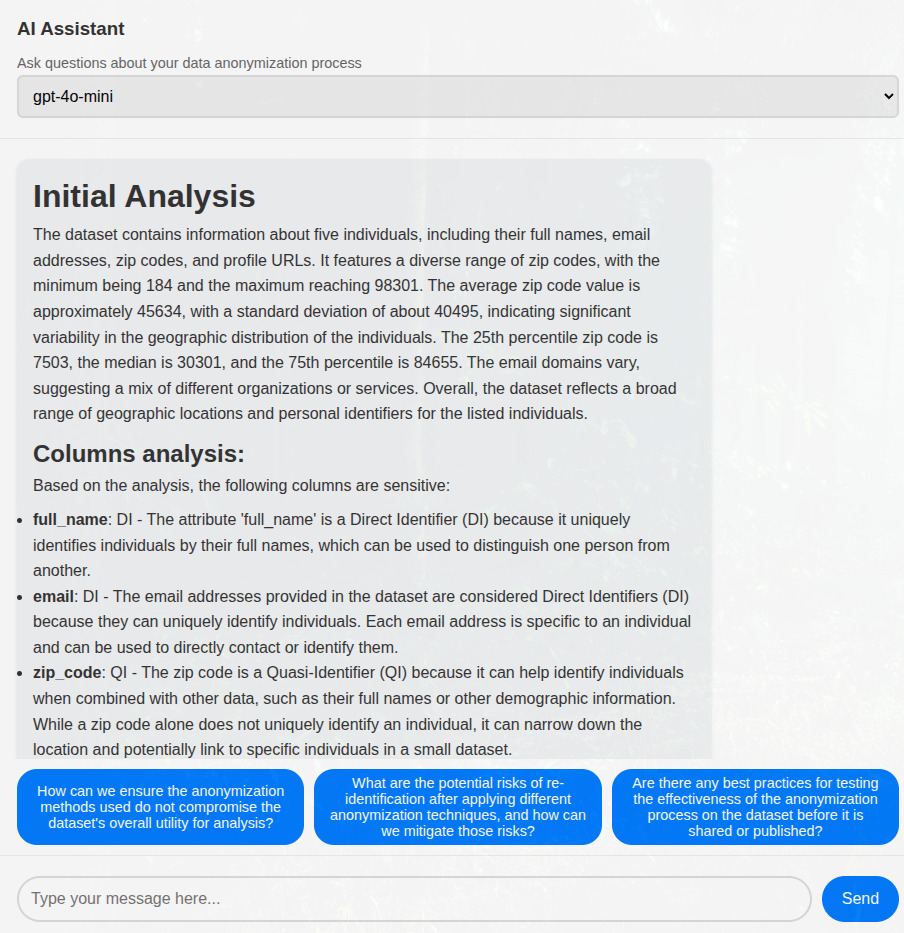
\includegraphics[height=9cm,width=0.85\linewidth,keepaspectratio]{images/chat_ui.jpg}
    \caption{Chat panel after the initial analysis.}
    \label{fig:ui-chat-results}
\end{figure}

A compact version of the results panel can be displayed on its own (Figure~\ref{fig:ui-table-only}).  
This view is intended for screenshots and future export to a report.

\begin{figure}[h]
    \centering
    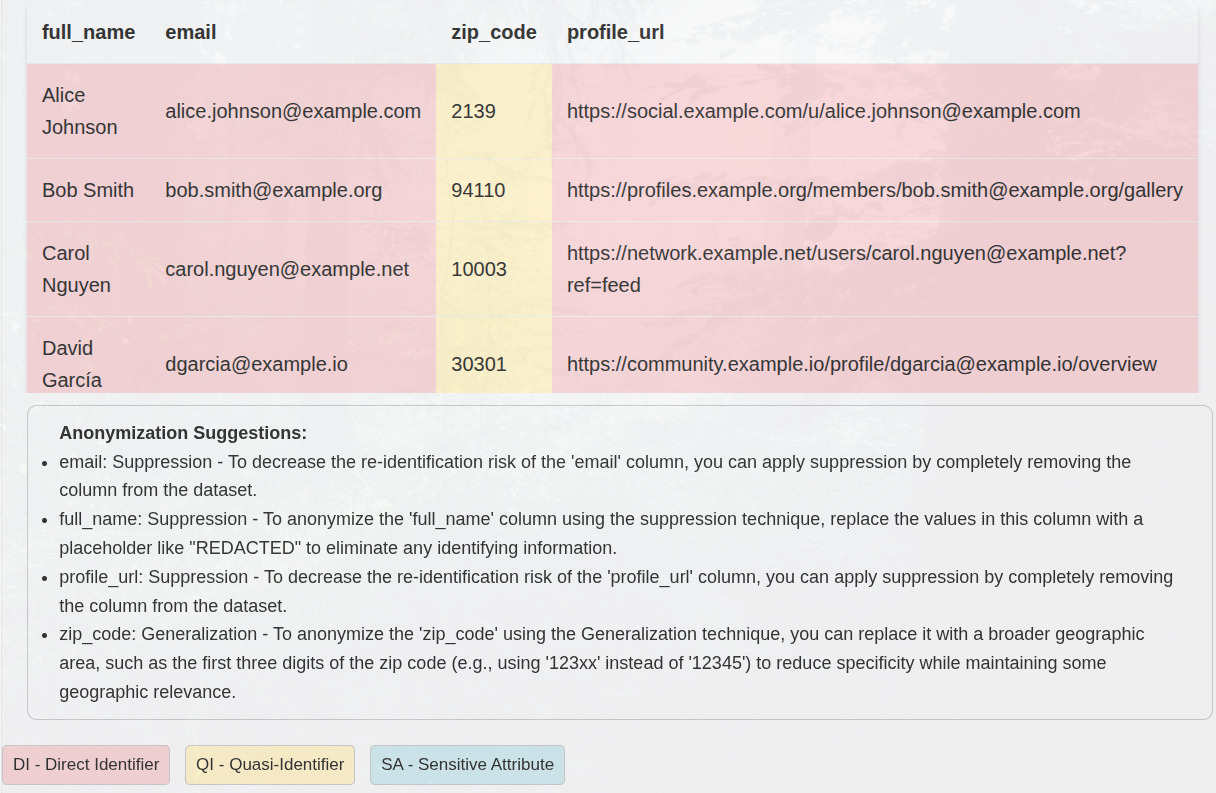
\includegraphics[width=0.85\linewidth,height=9cm,keepaspectratio]{images/results_ui.jpg}
    \caption{Standalone results panel with colour-coded table and suggestions.}
    \label{fig:ui-table-only}
\end{figure}

Interaction beyond this point is conducted entirely through the chat.  
No additional controls are required, which keeps the interface straightforward for users with varying technical backgrounds.


\section{Related Work}
\subsection{Application of LLM-Assisted Deductive Coding for Fuzzy Matching}

In our system, we implemented a \texttt{fuzzy\_match} function inspired by the deductive coding approach presented by Arnold et al. (2023) in \textit{LLM-Assisted Content Analysis}. Their methodology uses large language models (LLMs) to select a single best-fitting label from multiple predefined options, grounded in context and code definitions. We adapted this technique for robust, scalable option selection tasks in our pipeline.

\subsubsection{How We Used the Technique}

\paragraph{Problem Context}
Our task required selecting the most appropriate code or label for a given candidate input, from a predefined set of options, based on its meaning within a specific context. This is conceptually identical to deductive coding, where text data is categorized using an established codebook.

\paragraph{Inspiration from the Paper}
The paper demonstrated that LLMs perform effectively when prompted with:
\begin{itemize}
    \item An input text
    \item A list of options (codes) with clear definitions and examples
    \item Instructions to select the best fitting option only from the list
\end{itemize}
This structured prompt ensures the LLM leverages its semantic understanding to perform closed-set classification, avoiding invalid or out-of-scope outputs.

\paragraph{Our Implementation}
In our \texttt{fuzzy\_match} tool:
\begin{itemize}
    \item We provide the model with:
    \begin{itemize}
        \item A \textbf{context} explaining the selection task
        \item The \textbf{options dictionary}, mapping each code to its definition
        \item The \textbf{candidate input} requiring classification
    \end{itemize}
    \item We construct a structured prompt instructing the model to select the correct code strictly from the provided options.
    \item The LLM generates a JSON response containing:
    \begin{itemize}
        \item The selected \textbf{code}
        \item An optional \textbf{rationale} explaining its choice
    \end{itemize}
\end{itemize}

This mirrors the paper's method, where the LLM’s reasoning is grounded in the definitions and examples given for each code, allowing it to perform classification based on semantic alignment rather than purely lexical similarity.

\subsubsection{Key Principle Applied}


\textbf{Closed-set selection with definitions.} The technique enforces that the output is always within the valid set of codes, ensuring interpretability, consistency, and compatibility with downstream processing pipelines. This is critical for tasks such as qualitative coding, label assignment, or controlled classification where outputs outside the predefined set are invalid.

\subsection{Inspiration from JarviX}

Our LLMANO‑2 system draws inspiration from \textit{JarviX} , a no-code platform for tabular data analytics using LLMs. JarviX elegantly combines structured workflows, prompt-engineering logic, and AutoML integration to guide users through complex analytic tasks. We adopted several of its key design elements:

\begin{itemize}
    \item \textbf{LLM-driven, context-aware prompt flow.} As in JarviX, our system assesses the dataset schema and user goals to generate guiding questions and suggest relevant next actions dynamically .

    \item \textbf{Missing-context queries.} When crucial information is not provided, LLMANO‑2 automatically asks follow-up questions—mirroring JarviX’s Question Matcher module that detects ambiguity and clarifies requirements before analysis execution.
    \item \textbf{Future prompt suggestions.} Inspired by JarviX’s Analysis Consultant, which recommends subsequent lines of inquiry and visualizations, LLMANO‑2 likewise offers users a menu of potential follow-up prompts to deepen insight.
    \item \textbf{Hierarchical system architecture.} We adopted a modular architecture similar to JarviX’s pipeline decomposition—starting from data ingestion, to LLM-driven interpretation, to visualization and optimization—enabling flexible extension and improved maintainability.
\end{itemize}

\paragraph{Workflow (adapted from JarviX Figure 2).}
Figure 2 in the JarviX paper \cite{jarvix} illustrates their overall workflow architecture, comprising dataset analysis, prompt-based context extraction, and structured decision modules in sequence. We adapt this architecture to our own anonymization pipeline, where:
\begin{itemize}
    \item Dataset ingestion corresponds to JarviX's Data Parser.
    \item Our column classification and anonymization recommendation steps parallel their Prompting-based Analysis and AutoML modules.
    \item Follow-up prompt suggestions mirror JarviX's Analysis Consultant for next-action guidance.
\end{itemize}
We maintain their hierarchical decomposition but tailor each module to the privacy domai

\paragraph{Prompt logic.}
Let $\mathcal{D}$ be the dataset schema and $u$ the user's initial prompt. JarviX first derives:
\[
\mathrm{ctx}_0 = \textit{Parser}(\mathcal{D}, u),
\]
then checks completeness:
\[
\textit{if } \mathrm{ctx}_0 \not\vdash \textit{sufficient} \text{ then ask }\Delta q,
\]
and iterates until $\mathrm{ctx}_k$ is sufficient. The final query is submitted to the LLM for execution. This controlled, looped clarification inspired our back-and-forth logic.

\paragraph{Summary.}
By adapting JarviX’s workflow, prompt refinement, and suggestion strategies, LLMANO‑2 gains structured dialog management and context-sensitive prompting—key to robust no-code analytics. We extended this foundation with advanced context tracking and conversational capabilities to enhance usability and reliability.
\subsection{Definitions and Notation Used in LLMANO (Based on SCORR)}

In developing LLMANO, we adopted the definitions, notation conventions, and assumptions from the paper \emph{Scoring System for Quantifying the Privacy in Re-Identification of Tabular Datasets (SCORR)} . Specifically, we use its classification of Direct Identifiers (DIs), Quasi-Identifiers (QIs), and Sensitive Attributes (SAs), as well as its formal dataset notation and risk analysis assumptions.

\paragraph{Notation.}
Let $n$ be the number of records, $m$ the number of QI attributes, and $p$ the number of distinct persons:
\[
\begin{array}{rl}
\text{Attributes} &= \{a_1, a_2, \ldots, a_{m+2}\} \\
\text{Person ID} &= a_1 \\
\text{QI} &= \{a_2, \ldots, a_{m+1}\} \\
\text{SA} &= a_{m+2}
\end{array}
\]
where $v_{ij}$ is the value of attribute $a_j$ in record $i$, with:
\[
\begin{array}{rl}
v_{i1} &= u_k \quad \text{(Person ID)} \\
QI_i &= \{v_{i2}, \ldots, v_{i,m+1}\} \\
SA_i &= v_{i,m+2}.
\end{array}
\]

\paragraph{Assumptions.}
LLMANO adopts SCORR’s assumptions that:
\begin{enumerate}
    \item The intruder knows the QI values of the target data subject.
    \item The intruder aims to infer the SA value associated with the target.
\end{enumerate}

\paragraph{Summary.}
These definitions, notation structures, and assumptions from \emph{Scoring System for Quantifying the Privacy in Re-Identification of Tabular Datasets} provide the foundation for LLMANO’s identifier recognition logic, privacy metric calculations, and risk analysis modules.

\section{Evaluation}
\label{evaluation}

\subsection{Method}

We assessed the quality of the model output against a human‐labelled gold standard.  
Four members of the project team independently annotated each dataset column as \texttt{DI}, \texttt{QI}, \texttt{SA} or \texttt{NI}.  
Annotators worked only with a JSON excerpt that contained the same information given to the language model: the column name, up to twenty unique values, and a short dataset summary.  
External tools such as \texttt{pandas} were not permitted, which kept the human baseline comparable with the LLM input.  
Disagreements were resolved by discussion until full consensus was reached.

\subsection{Model set-up}

All models followed the two-step procedure described in Section~\ref{sec:architecture}.  
First, the model classified each column; second, it selected one of three anonymisation options (generalisation, suppression, differential privacy) or \texttt{none}.  
Prompts were identical across runs, and temperature was set to~0.  
Where a model exposed a function-calling interface, the structured-output variant was used; otherwise the plain text version with JSON validation was applied.

\subsection{Datasets and tasks}

We evaluated three public tabular datasets—Adult, Census, and Titanic—under two usage scenarios: \textit{machine-learning training} (“ML”) and \textit{public release}.  
The scenario was provided to the model as additional context.  
Different scenarios matter because stricter privacy may be required for public release than for internal model training.

\subsection{Metrics}

Performance was measured with simple accuracy and macro F1, computed per column and averaged over the dataset.  
Macro F1 gives equal weight to the four label classes and balances precision and recall.

\subsection{Results}

Table~\ref{tab:llm_eval_grouped} summarises the scores.  
Accuracy ranged from 0.25 to 0.60, with macro F1 following the same trend.  
Larger or more recent models, such as \texttt{gpt-4o-mini} and \texttt{llama3-70b}, tended to outperform smaller checkpoints, especially on the Adult dataset.  
Performance was lower on Titanic, whose small size yields fewer examples per column and makes classification harder for both humans and models.  
No single model dominated across all tasks, which suggests that prompt and context design still play a major role.

\begin{table}[h!]
\centering
\small
\begin{tabular}{lllccl}
\toprule
\textbf{Model} & \textbf{Purpose} & \textbf{Dataset} & \textbf{Accuracy Classification} & \textbf{Accuracy Anonymization} \\
\midrule
\multirow{3}{*}{gemma3\_12b} & Ml & Census & 0.32 & 0.26 \\
 & \multirow{2}{*}{Public} & Adult & 0.40 & 0.27 \\
 &  & Census & 0.47 & 0.37 \\
\midrule
\multirow{3}{*}{gemma3\_27b} & Ml & Census & 0.53 & 0.58 \\
 & \multirow{2}{*}{Public} & Adult & 0.27 & 0.20 \\
 &  & Census & 0.42 & 0.42 \\
\midrule
\multirow{6}{*}{gemma3\_4b} & \multirow{3}{*}{Ml} & Adult & 0.47 & 0.27 \\
 &  & Census & 0.47 & 0.37 \\
 &  & Titanic & 0.42 & 0.08 \\
 & \multirow{3}{*}{Public} & Adult & 0.47 & 0.33 \\
 &  & Census & 0.47 & 0.47 \\
 &  & Titanic & 0.33 & 0.33 \\
\midrule
\multirow{6}{*}{gpt-4o-mini} & \multirow{3}{*}{Ml} & Adult & 0.60 & 0.47 \\
 &  & Census & 0.42 & 0.42 \\
 &  & Titanic & 0.33 & 0.17 \\
 & \multirow{3}{*}{Public} & Adult & 0.47 & 0.40 \\
 &  & Census & 0.42 & 0.42 \\
 &  & Titanic & 0.25 & 0.17 \\
\midrule
\multirow{6}{*}{llama3-70b-8192} & \multirow{3}{*}{Ml} & Adult & 0.40 & 0.33 \\
 &  & Census & 0.53 & 0.47 \\
 &  & Titanic & 0.42 & 0.08 \\
 & \multirow{3}{*}{Public} & Adult & 0.33 & 0.27 \\
 &  & Census & 0.47 & 0.47 \\
 &  & Titanic & 0.42 & 0.42 \\
\midrule
\multirow{6}{*}{llama3.1:8b} & \multirow{3}{*}{Ml} & Adult & 0.53 & 0.40 \\
 &  & Census & 0.53 & 0.42 \\
 &  & Titanic & 0.17 & 0.08 \\
 & \multirow{3}{*}{Public} & Adult & 0.47 & 0.40 \\
 &  & Census & 0.42 & 0.32 \\
 &  & Titanic & 0.17 & 0.08 \\
\midrule
\multirow{3}{*}{mistral\_7b} & Ml & Census & 0.42 & 0.42 \\
 & \multirow{2}{*}{Public} & Adult & 0.27 & 0.20 \\
 &  & Census & 0.37 & 0.32 \\
\bottomrule
\end{tabular}
\caption{Accuracy scores of each model across datasets and purposes, benchmarked against our hand label annotations.}
\label{tab:llm_eval_grouped}
\end{table}


DISCLAMER because the models returned an empty string we those values where rated as false therefore the lower accuracy for Anonymisation methods

Across all datasets, every model in Table~\ref{tab:llm_eval_grouped} performs better than the uniform–random baseline of 0.25 accuracy that would arise from guessing among four classes.  Figures~\ref{fig:col} and~\ref{fig:anonymization} show the same trend graphically.  We also note that \texttt{gpt-4o-mini} occasionally returned no anonymisation method for a column; each omission was treated as an error, which lowers its reported scores.



\newpage

\begin{figure}[!htbp]
    \centering
    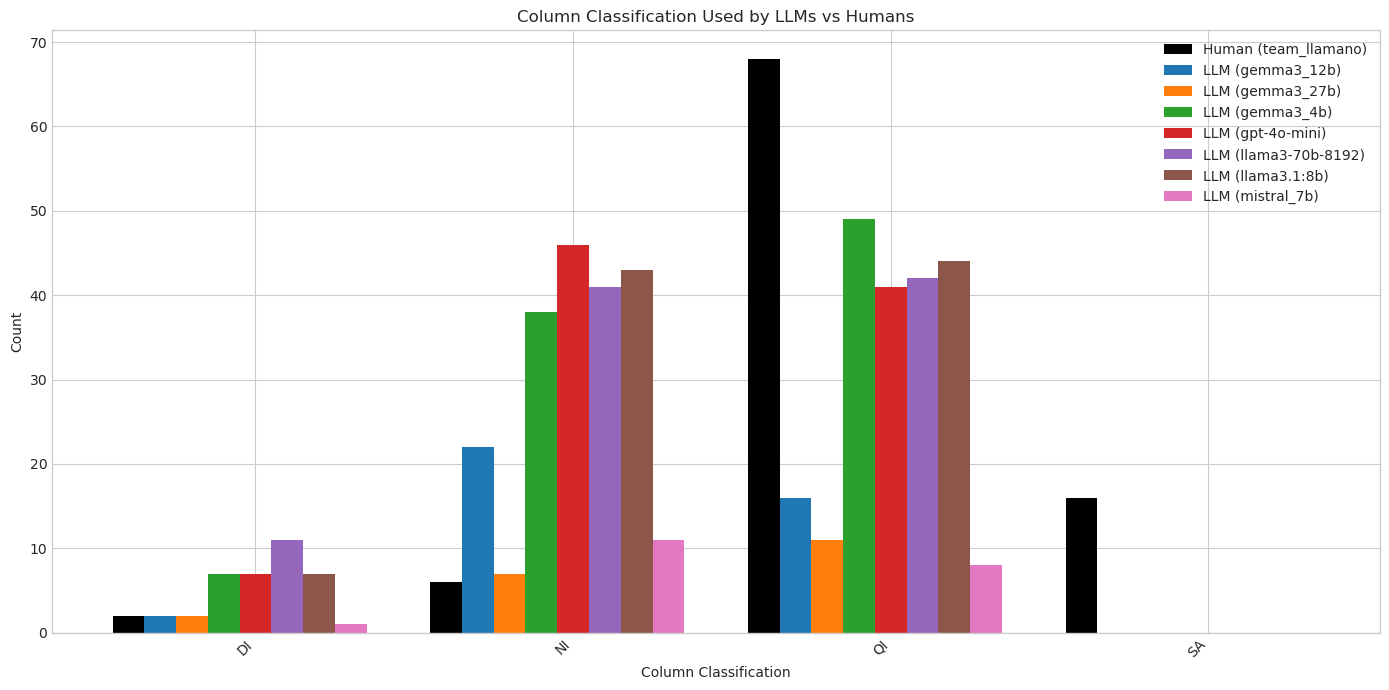
\includegraphics[width=\linewidth]{images/plot_eval2.png}
    \caption{Column classifications produced by human annotators and language models.}
    \label{fig:col}
\end{figure}

\begin{figure}[!htbp]
    \centering
    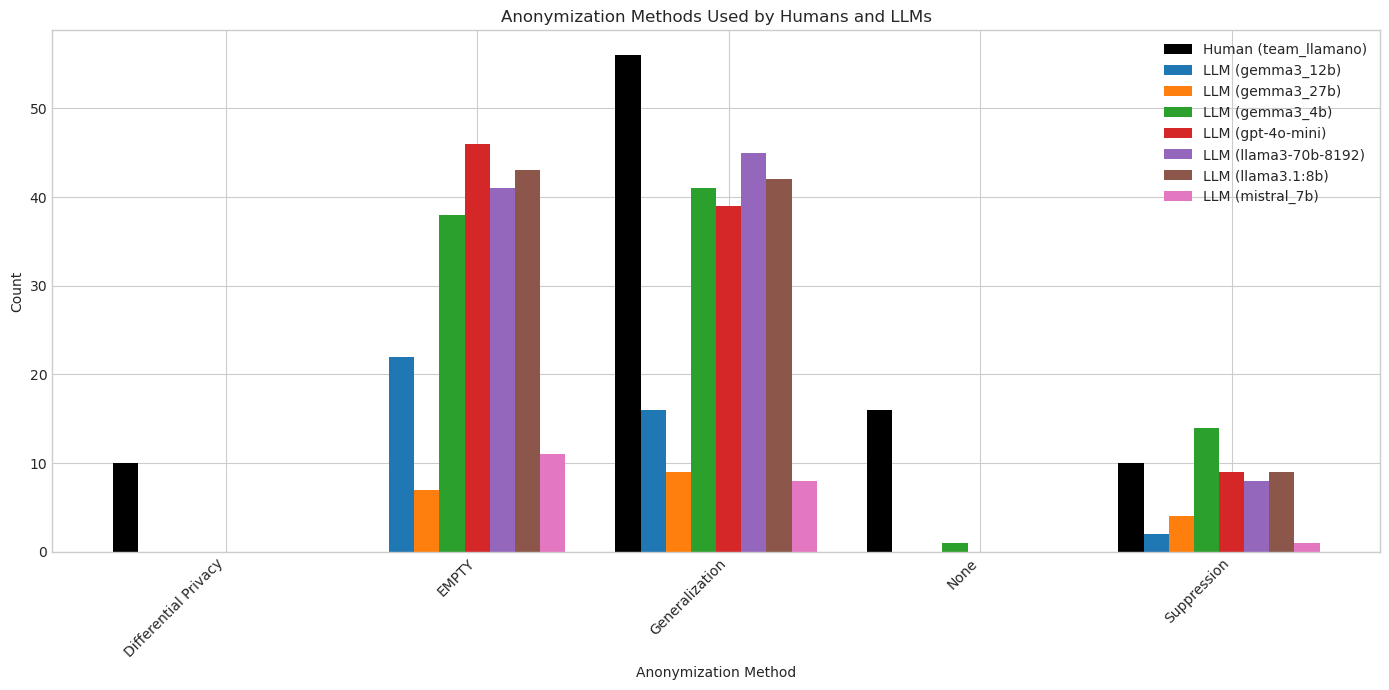
\includegraphics[width=\linewidth]{images/plot_eval.png}
    \caption{Anonymisation methods selected by human annotators and language models.}
    \label{fig:anonymization}
\end{figure}


In our evaluation, we first encountered the issue that some free LLM providers had pretty limiting rate limits. Due to time constraints, we had to skip testing Gemini. We mostly used Grok, OpenAI, and our own self-hosted O-LLaMA, which included a few local models. However, we could not test all models on everything, again due to the time limitations.

One discovery we made was that, for the anonymization method selection task, many models returned an empty result. This was either due to an error in our pipeline or, more likely, a behavioral issue where the models simply did not return the expected format. This disrupted our pipeline, and our error handling caught it and returned an empty result. So, this could reflect both a weakness in the LMs—failing to return the correct format, and some limitations in our pipeline, which may not have been robust enough. It could also be due to our prompts not being specific enough.

Interestingly, OpenAI, expected to be the most responsive to prompt formatting, had the most empty results. This might suggest a prompt issue, or perhaps some other deeper behavior worth investigating.

Another notable point is that differential privacy was never selected by the LMs. This could be due to the way we prompted, but also, from an annotator’s perspective, it was quite difficult to know when to apply it. We only selected it in the case of machine learning models when the context involved a number and it seemed appropriate. Even then, it was a difficult decision. So, it is not surprising that the LMs did not pick it, though we had hoped that at least for ML-related contexts they would. This may be a prompting issue as well, or perhaps differential privacy is too complex as an anonymization method, and not well represented in the training data of the LMs.

Another finding from Figure~\ref{fig:col}, is that no model ever classified anything as a sensitive attribute. That is something we may want to address in future versions of the pipeline. Perhaps refining the prompts, or switching to a two step process could help, first classify whether something is a direct identifier, indirect (quasi) identifier, or non-identifier, and then, for quasi-identifiers, return a “sensitive: true/false” flag or sensitivity score to make this dimension more prominent.

Among the anonymization techniques, generalization was selected the most by both humans and LMs. For suppression, the tendencies were similar, although we noticed that LLaMA 70B used it less often, as did Gemini 27B. So, it appears that the more capable models tend to use suppression less, which is an interesting observation.

In Figure~\ref{fig:col}, LLaMA 70B also seemed to classify more entities as direct identifiers. And from Table~\ref{tab:llm_eval_grouped}, we can see that the F1 score of the o4-mini model is the highest, making it the best model overall, even though its accuracy is not as high.
\section{Discussion}
\subsection{Limitations}
\label{sec:limitations}

The present prototype demonstrates the feasibility of an LLM–assisted anonymisation workflow, yet several constraints remain.  
First, the system relies on multiple, narrowly scoped prompts to achieve stable results.  Each additional prompt increases latency and, when a commercial model is used, raises monetary cost through higher token throughput.  A production deployment will therefore require a careful balance between prompt granularity and operational expense.  

Second, although the architecture permits arbitrary Python tools to be exposed to the language model, only a small set is currently implemented, limited to basic privacy metrics such as $k$-anonymity and $l$-diversity.  Expanding this library is essential for broader applicability.  

Third, the range of supported anonymisation techniques is still narrow.  At present the system can recommend generalisation, suppression and a differential-privacy layer, but it cannot yet prescribe more advanced transformations such as homomorphic encryption, local differential privacy or synthetic data generation.  A systematic comparison with these alternatives is left for future work.  

Finally, the current output is minimal.  Results appear only as a simple, chat-independent box that lists one suggested anonymisation method per attribute, and they are not yet downloadable in any report format.  The box is meant as a symbolic placeholder for a richer document that the LLM will ultimately compose, containing a narrative summary, detailed rationale and actionable next steps.  Implementing export functions and an editable report view remains future work.

\subsection{Future work}

Although LLMANO-2 already provides a flexible and modular setup for LLM-assisted anonymization, there is still plenty of room to grow and improve. Two areas stand out as especially promising for future development which are integrating open-source agentic frameworks, and moving away from heavy prompt engineering in favor of Retrieval-Augmented Generation (RAG) to support more scalable and efficient reasoning.

\paragraph{Agentic Orchestration and Structured LLM Tooling.}
As LLMs become more deeply embedded in structured applications, there is growing momentum behind the so-called “agentic” systems. Setups where models do not just respond to prompts, but also take initiative, call tools, and manage multi-step workflows. Open-source frameworks like LangChain and CrewAI make this kind of functionality much easier to implement. For LLMANO-2, a natural next step would be to adopt these frameworks to handle tool-calling and decision-making more explicitly. Features like LangChain’s StructuredOutput and StateGraph could allow the system to coordinate complex tasks, such as risk analysis, column classification, and technique selection in a clean, modular way. This would move the workflow beyond a simple sequence of prompts into a flexible decision graph, making it easier to track, reuse, and extend each step of the process.

In addition, structured function-calling, supported by LangChain and similar agentic frameworks, lets us enforce strict output formats in a way that simple prompt validation often can not. This shifts the role of the LLM from just a reasoning engine to something closer to a programmable agent that can reliably carry out specific steps in the anonymization workflow. With tool-calling, the model could directly trigger external components like homomorphic encryption libraries or advanced generalization tools, without needing to encode all the logic in the prompt itself. This kind of structured setup fits well with modern hybrid AI practices, where symbolic routines and modular code work alongside probabilistic models to create more reliable and maintainable systems \cite{jarvix}.

\paragraph{From Prompting to Retrieval-Augmented Generation (RAG).}
Currently, LLMANO-2 depends heavily on carefully crafted prompts to guide its anonymization logic and provide context. While this approach has produced good results, it is also resource intensive, both in terms of token usage and the effort needed to maintain the prompts. A more scalable alternative is Retrieval-Augmented Generation (RAG), which separates the retrieval of relevant information from the actual generation process. Instead of packing all the logic into a single prompt, a RAG-based system can pull in relevant anonymization strategies, definitions, and examples from a vector store, allowing the model to work with just the most useful context for each task.

In a RAG-based setup, the choice of which anonymization method to use would be informed by embedded representations of past successful cases, legal requirements, and established best practices, all stored in a well curated knowledge base. This approach is especially useful when working across different domains like healthcare, finance, or education, where privacy expectations can vary widely. Tools like FAISS \cite{faiss2023} or Chroma can serve as the vector search engine behind this, enabling the system to retrieve relevant context without being limited by token constraints. Combined with LLM reasoning, this setup can improve both accuracy and reliability by grounding the model’s output in meaningful, domain-specific information \cite{llm_content_analysis}.

Adopting a RAG-based architecture would also make the system more modular. Domain-specific privacy guidelines could be stored in separate knowledge bases, allowing the model to retrieve only what’s relevant for each context, without needing to retrain or manually tweak prompt templates. This is particularly helpful when dealing with evolving regulations, like updates to GDPR interpretations, since changes can be made directly in the documents rather than in the application code.

\paragraph{Downloadable, model-generated reports.}
At present the system surfaces its findings only inside the chat window; users cannot export a consolidated document.  
A practical extension is a “Generate report” action that compiles the conversation’s key artefacts (dataset summary, column classifications, risk metrics and recommended transformations) into a standalone PDF or HTML file.  
The report would follow a fixed template populated by the LLM and post-processed with \texttt{pandoc} or \texttt{LaTeX}, guaranteeing a stable layout while allowing the model to fill narrative sections such as methodological notes or next-step check-lists.  
A download link should appear in the interface once generation is complete.  
Longer term, the report could be made editable: users would request revisions in natural language, the LLM would patch the underlying markdown, and a new version would be rendered on demand.  
This feature closes the loop between interactive guidance and formal documentation, giving practitioners a tangible artefact for audit trails, compliance submissions or further manual refinement.


\paragraph{Summary.}
Agentic orchestration and RAG complement each other well and offer solutions to two of LLMANO-2’s current limitations, its reliance on linear prompt flows and the brittleness of static prompt design. By combining tool-based reasoning with modular knowledge retrieval, the system could become more robust, easier to interpret, and better suited for scaling. These improvements would also support more interactive, human-in-the-loop workflows, where users can review, adjust, or fine-tune anonymization steps based on clear intermediate outputs.

Ultimately, future versions of LLMANO should aim to move beyond static prompt execution and become proactive, memory-enhanced agents capable of retrieving context on demand, planning anonymization strategies, calling tools as needed, and adapting flexibly to new domains and evolving privacy requirements.


\section{Conclusion}
\label{sec:conclusion}

This report presented LLMANO, a prototype that combines large language models with a lightweight, modular framework for column level anonymization guidance. The system accepts a CSV dataset, applies an automatic screening based on a fixed codebook, and proposes one anonymisation strategy per attribute. All components are deployable on-premise, and the system is designed to remain model-agnostic, new language models or privacy tools can be integrated simply by adding an adapter. This allows LLMANO to evolve alongside emerging technologies without requiring substantial redesign.

The results of our evaluation demonstrate that LLMs are capable of providing meaningful classification of dataset attributes into privacy relevant categories (DI, QI, SA, NI), and of suggesting anonymisation strategies that align with common best practices. Across multiple public datasets, LLMANO achieved promising accuracy and macro F1 scores when benchmarked against human-labeled gold standards. These findings suggest that a semi-automated, LLM assisted approach can substantially reduce the manual effort typically required for dataset anonymisation, particularly for non-experts.

Nevertheless, the current implementation has several limitations. Only three anonymisation techniques, generalisation, suppression, and differential privacy, are currently supported, and the set of privacy metrics remains small. Furthermore, the interface does not yet support downloadable reports or more advanced visualisations of privacy risks. These features are essential for real world deployment, especially in regulated environments where auditability and traceability are key.

Looking forward, future iterations of LLMANO could benefit from integration with agentic frameworks and Retrieval-Augmented Generation (RAG), which would allow the system to retrieve relevant legal guidelines, prior cases, or domain-specific knowledge on demand. This would make the anonymisation recommendations more context aware, flexible, and robust. Exportable, editable reports and a richer user experience would also enhance the tool’s value in professional settings.

In sum, LLMANO-2 represents a step toward practical, intelligent anonymisation support for tabular data. It validates that LLMs can assist in making privacy decisions that respect both legal requirements and data utility, without exposing raw data or demanding deep technical expertise from the user. While much is still to be done, the system provides a strong foundation for future development in privacy aware data publishing and opens up new possibilities for trustworthy, explainable anonymisation workflows.

\begin{thebibliography}{9}

\bibitem{li2018}
N.~Li \emph{et~al.},
“On sampling, anonymization, and differential privacy…,”
\emph{IEEE Trans.\ Knowledge and Data Engineering}, 2018.
\href{https://www.tandfonline.com/doi/full/10.1080/17579961.2018.1452176#abstract}{%
\texttt{doi:10.1080/17579961.2018.1452176}
}

\bibitem{esser2023}
E.~Esser \emph{et~al.},
“Privacy attacks on LLMs and how to defend,”
\emph{Science Advances}, 2023.
\href{https://www.science.org/doi/full/10.1126/sciadv.adn7053}{%
\texttt{doi:10.1126/sciadv.adn7053}
}

\bibitem{fake_news_dataset}
Clément Bisaillon,
\emph{Fake and Real News Dataset}. Kaggle.
\href{https://www.kaggle.com/datasets/clmentbisaillon/fake-and-real-news-dataset}{https://www.kaggle.com/datasets/clmentbisaillon/fake-and-real-news-dataset}

\bibitem{lending_club_dataset}
Wordsforthewise,
\emph{Lending Club Dataset}. Kaggle.
\href{https://www.kaggle.com/datasets/wordsforthewise/lending-club/data}{https://www.kaggle.com/datasets/wordsforthewise/lending-club/data}

\bibitem{student_demographics_dataset}
Anıl Gürbüz,
\emph{Student Demographics – Online Education Dataset}. Kaggle.
\href{https://www.kaggle.com/datasets/anlgrbz/student-demographics-online-education-dataoulad}{https://www.kaggle.com/datasets/anlgrbz/student-demographics-online-education-dataoulad}

\bibitem{hospital_discharges_dataset}
Bhautik Mangukiya,
\emph{Hospital Inpatient Discharges Dataset}. Kaggle.
\href{https://www.kaggle.com/datasets/bhautikmangukiya12/hospital-inpatient-discharges-dataset}{https://www.kaggle.com/datasets/bhautikmangukiya12/hospital-inpatient-discharges-dataset}

\bibitem{adult_income_dataset}
UCI Machine Learning Repository,
\emph{Adult Census Income Dataset}. Kaggle.
\href{https://www.kaggle.com/datasets/uciml/adult-census-income/data}{https://www.kaggle.com/datasets/uciml/adult-census-income/data}

\bibitem{titanic_dataset}
Yasser Hatab,
\emph{Titanic Dataset}. Kaggle.
\href{https://www.kaggle.com/datasets/yasserh/titanic-dataset}{https://www.kaggle.com/datasets/yasserh/titanic-dataset}

\bibitem{machanavajjhala2007}
Machanavajjhala, A., Kifer, D., Gehrke, J., and Venkitasubramaniam, M.,
\emph{$l$-diversity: Privacy beyond $k$-anonymity}. ACM Transactions on Knowledge Discovery from Data (TKDD), 1(1), 2007.
\href{https://doi.org/10.1145/1217299.1217302}{https://doi.org/10.1145/1217299.1217302}

\bibitem{li2007tcloseness}
Li, N., Li, T., and Venkatasubramanian, S.,
\emph{$t$-Closeness: Privacy beyond $k$-anonymity and $l$-diversity}. In Proceedings of the 23rd International Conference on Data Engineering (ICDE), 2007, pp. 106–115.
\href{https://doi.org/10.1109/ICDE.2007.367856}{https://doi.org/10.1109/ICDE.2007.367856}

\bibitem{fung2010survey}
Fung, B. C. M., Wang, K., Chen, R., and Yu, P. S.,
\emph{Privacy-preserving data publishing: A survey of recent developments}. ACM Computing Surveys (CSUR), 42(4), 2010, Article 14.
\href{https://doi.org/10.1145/1749603.1749605}{https://doi.org/10.1145/1749603.1749605}





\bibitem{llm_content_analysis}
Gong, M., Choudhury, S. R., Jiang, M., He, Y., Meng, Y., Li, X., Zhang, C., and Liu, H.,
\emph{LLM-Assisted Content Analysis: Demonstration and Evaluation}. arXiv preprint arXiv:2306.14924, 2023.
\href{https://arxiv.org/abs/2306.14924}{https://arxiv.org/abs/2306.14924}

\bibitem{scorr_paper}
Folz, J., Vidanalage, M. D., Aufschläger, R., Almaini, A., Heigl, M., Fiala, D., and Schramm, M.,
\emph{Scoring System for Quantifying the Privacy in Re-Identification of Tabular Datasets}. IEEE Access, 2025.
\href{https://ieeexplore.ieee.org/document/10973096}{https://ieeexplore.ieee.org/document/10973096}

\bibitem{jarvix}
Liu, S., Ji, Y., Tan, S., Zhang, J., Zhao, W., Liu, S., Chen, M., and Hu, Z.,
\emph{JarviX: An LLM No-code Platform for Tabular Data Analysis and Optimization}. arXiv preprint arXiv:2312.02213, 2023.
\href{https://arxiv.org/abs/2312.02213}{https://arxiv.org/abs/2312.02213}



\end{thebibliography}
\end{document}

